\documentclass[dvipsnames]{beamer} %dvipsnames gives pre-defined colors!

%%%%%%%%%%%%%%%%%%%%%%%%%%%%%%%%%%%%%%%%%%%%%%%%%%
%%%%%%%%%%%%%%%%%   PREAMBLE   %%%%%%%%%%%%%%%%%%%
%%%%%%%%%%%%%%%%%%%%%%%%%%%%%%%%%%%%%%%%%%%%%%%%%%

\usetheme{ppt2003}

\usepackage{amsmath}
\usepackage{graphicx}

%for \XeLaTex command
\usepackage{xltxtra} 

%for the checkmark sign
\usepackage{tikz}
\def\checkmark{\tikz\fill[scale=0.2](0,.35) -- (.25,0) -- (1,.7) -- (.25,.15) -- cycle;}

% define some colors
\newcommand{\upcolor}{RoyalBlue}
\newcommand{\downcolor}{BrickRed}

%title page
\title{A PPT2003 Style Template}
\author[\c{S}an G\"{u}ltekin]{\c{S}an G\"{u}ltekin}
\titlegraphic{\includegraphics[scale=.12]{figures/logo_columbia.png}}
\institute{Columbia University}
\date[\today]{\today}

%%%%%%%%%%%%%%%%%%%%%%%%%%%%%%%%%%%%%%%%%%%%%%%%%%
%%%%%%%%%%%%%%%%%   SLIDES   %%%%%%%%%%%%%%%%%%%%%
%%%%%%%%%%%%%%%%%%%%%%%%%%%%%%%%%%%%%%%%%%%%%%%%%%

\begin{document}



\begin{frame}
\titlepage
\end{frame}



\begin{frame}
\frametitle{About this template}
\begin{itemize}
	\item This is a custom beamer template you can use for presentations.
	\item It is based on one of the frequently used layouts in Microsoft's PowerPoint 2003!
	\item As the first step I drew the layout in Adobe Illustrator; you can find this in the file ``ppt2003.pdf''.
	\item This vector image is then used in the style file ``beamerthemeppt2003.sty'' which specifies the layout.
	\item You can change the style file as you desire.
	\item The fonts I use are ``Impact'' for the titles and ``Times New Roman'' for the text. This utilizes the \texttt{fontspec} package so I recommend you compile with \XeLaTeX.
\end{itemize}
\end{frame}



\begin{frame}
\begin{center}
\frametitle{You can add an outline slide like this}
\noindent\fbox{%
    \parbox{3.5in}{%
    	\begin{center}
        	Part I: Introduction
        \end{center}
    }%
} \\
\vspace{.1in}
\noindent\fbox{%
    \parbox{3.5in}{%
    	\begin{center}
        	Part II: New Results
        \end{center}
    }%
} \\
\vspace{.1in}
\noindent\fbox{%
    \parbox{3.5in}{%
    	\begin{center}
        	Part III: Conclusion
        \end{center}
    }%
}
\end{center}
\end{frame}



\begin{frame}
\frametitle{Colors}
I also define \textcolor{\upcolor}{two} \textcolor{\downcolor}{colors} to highlight important things. You can add more colors but I personally prefer a two-color scheme.\\
\vspace{.1in}
For example:\\
\textcolor{\upcolor}{\checkmark{} This is an advantage.}\\
\textcolor{\upcolor}{\checkmark{} This is an advantage.}\\
\textcolor{\upcolor}{\checkmark{} This is an advantage.}\\
\textcolor{\downcolor}{$\times$ This is a disadvantage.}\\
\textcolor{\downcolor}{$\times$ This is a disadvantage.}\\
\textcolor{\downcolor}{$\times$ This is a disadvantage.}\\
\end{frame}



\begin{frame}
\frametitle{Math typeset}
While I use Times New Roman for the text, I keep the Computer Modern Serif font for the equations, which gives the traditional \LaTeX{} look-and-feel. To illustrate this, the multivariate Gaussian distribution is given by
\begin{align*}
	p(x) = (2\pi)^{-d/2} |\Sigma|^{-1/2} \exp \left\{ -\frac{1}{2} (x-\mu)^\top \Sigma^{-1} (x-\mu) \right\}
\end{align*}
\end{frame}



\begin{frame}
\frametitle{You can add a figure like this}
\begin{center}
	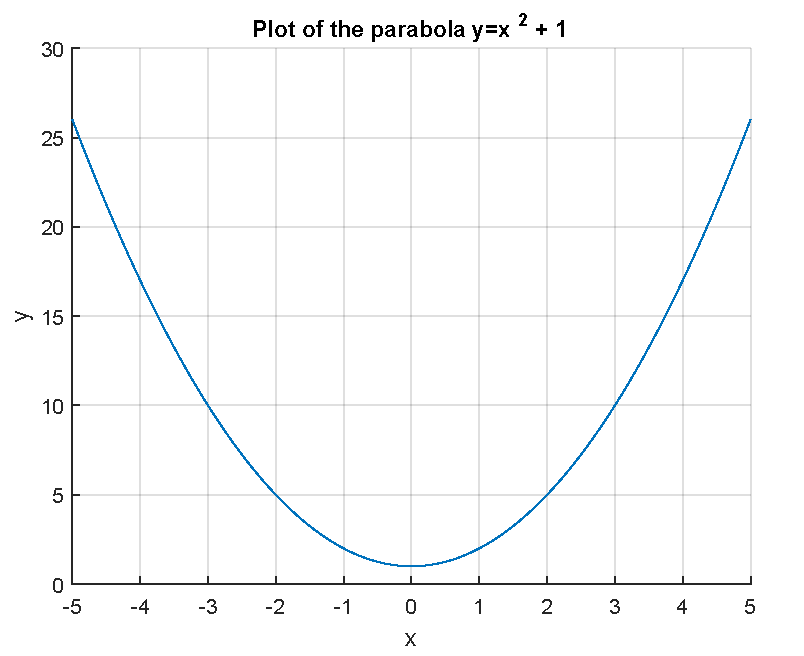
\includegraphics[scale=.45]{figures/parabola.pdf}
\end{center}
\hrule
\vspace{.1in}
That's it!\\
\vspace{.1in}
If you have more questions, contact me: \texttt{san.gultekin@gmail.com}
\end{frame}



\end{document}